\hypertarget{section-system-scope-and-context}{%
\section{3 System Scope and Context}\label{section-system-scope-and-context}}

\textbf{Contents}

This section defines the scope and context of the Webshop system, a platform designed to display products to users, process payments, and confirm orders. The system retrieves product data from an Azure-hosted database, integrates with Stripe for payment processing, and uses an Azure email service to send order confirmations. It outlines the external entities—users, the Azure database, Stripe, and the Azure email service—and specifies the business and technical interfaces connecting them to the Webshop.

\textbf{Motivation}

Understanding the Webshop's and its external entities' interfaces is crucial for stakeholders to make informed architectural decisions. Clear boundaries ensure alignment on what the system handles (e.g., product display and payment) versus what it relies on externally (e.g., payment processing via Stripe), guiding both development and deployment decisions.

\textbf{Form}

The business context will be presented with a context diagram showing the Webshop as a black box linked to its external partners, alongside a table listing communication partners, inputs, and outputs. The technical context will use a UML deployment diagram to illustrate the system’s technical connections, supplemented by a mapping table tying domain inputs/outputs to specific channels.

\hypertarget{_business_context}{%
\subsection{Business Context}\label{_business_context}}

\textbf{Contents}

The Webshop system interacts with several external entities: (1) Users, who browse products, submit orders, provide payment information, and receive order confirmations; (2) Azure-hosted Database, which provides product data; (3) Stripe, which processes payment transactions; and (4) Azure Email Service, which delivers order confirmation emails. This subsection specifies the domain-specific inputs and outputs exchanged between the Webshop and these partners.

\textbf{Motivation}

Defining these interactions ensures stakeholders understand the Webshop’s core business functions—displaying products, processing orders, and confirming purchases—and its dependencies on external systems for data, payments, and notifications.

\textbf{Form}

The context diagram below depicts the Webshop system and its external interactions. The table details the inputs and outputs for each communication partner.

\begin{figure}[h]
  \centering
  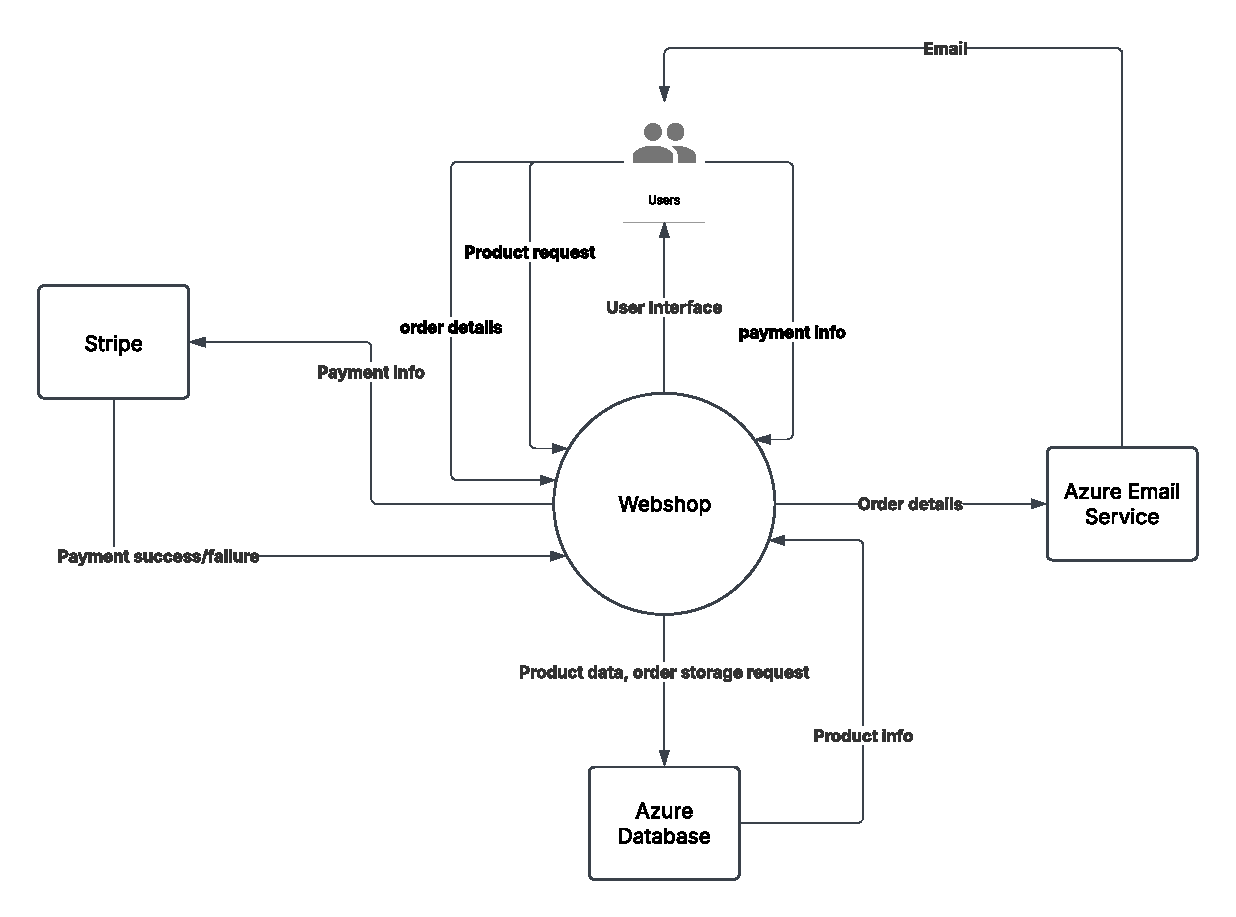
\includegraphics[width=0.8\textwidth]{images/webshop_context_diagram.pdf} 
  \caption{Context Diagram of the Webshop System and Its External Entities}
  \label{fig:webshop-context}
\end{figure}

\begin{table}[h]
  \centering
  \resizebox{\textwidth}{!}{%
    \begin{tabular}{|l|l|l|}
      \hline
      Communication Partner & Inputs                          & Outputs                           \\
      \hline
      Users                & User Interface & Product requests, order details, payment info \\
      Azure Database       & Product data, order storage requests & Product info \\
      Stripe               & Payment info                   & Payment success/failure response \\
      Azure Email Service  & Order details                  & email delivered to users \\
      \hline
    \end{tabular}
  }
  \caption{Inputs and Outputs for Webshop Communication Partners}
  \label{tab:webshop-business-context}
\end{table}

\hypertarget{_technical_context}{%
\subsection{Technical Context}\label{_technical_context}}

\textbf{Contents}

This subsection details the technical interfaces connecting the Webshop system to its environment, including the channels, protocols, and hardware used. The Webshop operates as a web application hosted on Azure, communicating with users via HTTP/HTTPS over the internet, accessing the Azure-hosted Database through REST API calls, integrating with Stripe via HTTPS for payment processing, and utilizing Azure Email Service for SMTP-based email delivery. It maps these technical connections to the business inputs and outputs described in the Business Context.

\textbf{Motivation}

Understanding these technical interfaces is critical for infrastructure designers and developers to ensure reliable connectivity, secure data transmission, and scalable deployment of the Webshop. It informs decisions about hosting, network configuration, and integration with external services like Stripe and Azure.

\textbf{Form}

The UML deployment diagram below illustrates the Webshop’s technical architecture and its connections to external entities. The table maps the domain-specific inputs and outputs to their technical channels and protocols.

\begin{figure}[h]
  \centering
  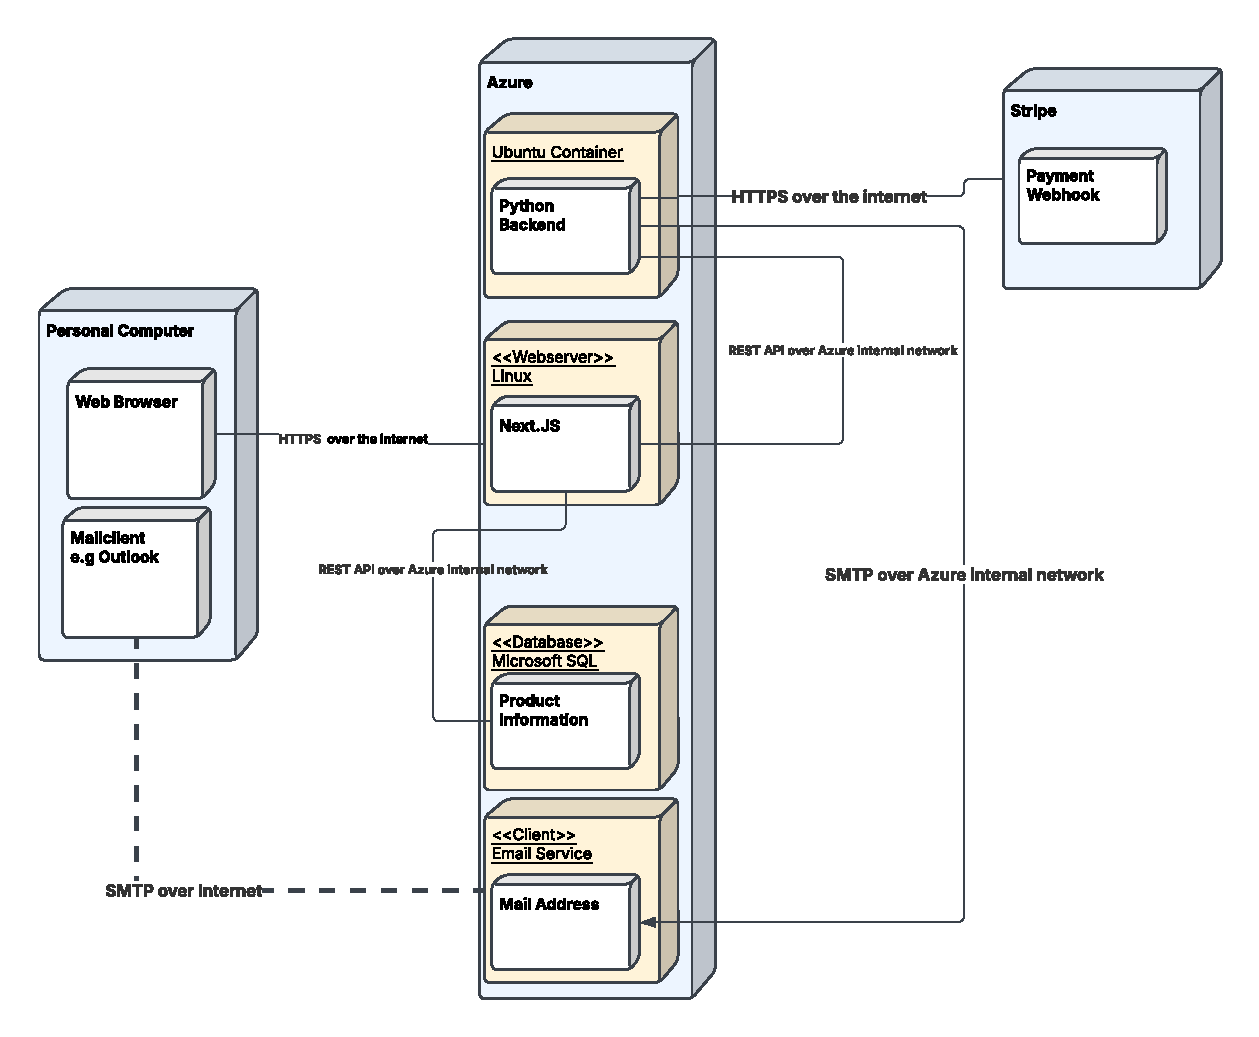
\includegraphics[width=0.8\textwidth]{images/webshop_deployment_diagram.pdf} 
  \caption{UML Deployment Diagram of the Webshop Technical Architecture}
  \label{fig:webshop-deployment}
\end{figure}

\begin{table}[h]
  \centering
  \resizebox{\textwidth}{!}{%
    \begin{tabular}{|l|l|l|}
      \hline
      Input/Output                          & Channel/Protocol               & Description (Optional)                   \\
      \hline
      Product requests, order details, payment info (Users → Webshop) & HTTPS over the Internet        & User interactions via web browser       \\
      Product listings, order confirmation (Webshop → Users) & HTTPS over the Internet        & Web app responses                        \\
      Product data, order storage requests (Webshop → Azure Database) & REST API over Azure internal network & Database queries and updates            \\
      Product info (Azure Database → Webshop) & REST API over Azure internal network & Data retrieval for product display      \\
      Payment info (Backend → Stripe)       & HTTPS over the Internet        & Payment processing requests             \\
      Payment webhook (Stripe → Backend)    & HTTPS over the Internet        & Payment status updates via webhook       \\
      Order details (Webshop → Azure Email Service) & SMTP over Azure internal network & Email notification setup                \\
      Email delivered to users (Azure Email Service → Users) & SMTP over Internet             & Email delivery to users                 \\
      \hline
    \end{tabular}
  }
  \caption{Mapping of Webshop Inputs/Outputs to Technical Channels}
  \label{tab:webshop-technical-mapping}
\end{table}
